\documentclass[aspectratio=169,10pt]{beamer}
\usepackage{teaching_slides}


% \usepackage{lipsum}
% \usepackage{amsmath} 
% \usepackage{amsthm} 
% \usepackage{amssymb} 
% \usepackage{mathtools}
% %\usepackage{natbib}
% \usepackage{dutchcal}


% \newcommand{\vect}[1]{\symbf{\symbf{#1}}}
% \newcommand{\pd}[2]{\frac{\partial{#1}}{\partial{#2}}}
% \newcommand{\expect}[2]{\mathbb{E}_{#1}\left[{#2}\right]}
% \newcommand{\expectsmall}[2]{\mathbb{E}_{#1}{#2}}
% \newcommand{\expectsuper}[3]{\mathbb{E}_{#1}^{#2}\left[{#3}\right]}
% \newcommand{\ind}[1]{\mathbbm{1}\left\{{#1}\right\}}
% \newcommand{\prob}[1]{\mathbb{P}\left\{{#1}\right\}}
% \newcommand{\derivative}[2]{\frac{d{#2}}{d{#1}}}
% \newcommand{\cat}[1]{\citeasnoun{#1}}

% title page
% title page
\title{What's new in Micro Data?}
\author{Chris Conlon}
\institute{NYU Stern}
\date{Fall 2025}





\begin{document}



%--------------
% TITLE PAGE
\begin{frame}
\titlepage
\end{frame}


\section*{What's new with micro data?}

\begin{frame}{Micro Data: Motivation}
Data are a lot better than they were in 1995. It is common to observe:
\begin{itemize}
\item Choices of individuals, demographic characteristics, etc.
\begin{itemize}
\item Examples: Nielsen Panelist Data, Kantar Worldpanel, IRI, etc.
\end{itemize}
\item Higher frequency data, now $M_t \rightarrow \infty$ may not be a good assumption.
\begin{itemize}
    \item Not every product gets purchased every hour or every day.
    \item Examples: Taxis/Uber, Daily airline bookings, hotel stays, AirBnB, Amazon, etc.
\end{itemize}
\end{itemize}
How can we make the best use of the data that we see?
\end{frame}


\begin{frame}{Common Approaches}
\begin{enumerate}
\item Use control function approach of Petrin and Train (2010)
\item Fully specifiy likelihood with a parametric assumption on $f(\xi)$ (Jiang Machanda Rossi (2009))
\item Add ``micro-moments'' a la Petrin (2001) or Micro BLP (2004) but otherwise aggregate data.
\begin{itemize}
\item How do we choose them? Are we throwing away information?
\end{itemize}
\item Add aggregate data moments to maximum likelihood (Grieco, Murry, Pinkse, Sagl 2023)
\end{enumerate}
\end{frame}


\begin{frame}{Petrin Train (2010): Control Functions}
\begin{align*}
u_{ijt} &=  \beta_i\, x_{jt} - \alpha_i p_{jt} + \xi_{jt} + \varepsilon_{ijt} \\
p_{jt} &= f(x_{jt}, z_{jt}) + e_{jt}\\
\xi_{jt} &= \lambda e_{jt} + \zeta_{jt}  \text{ with } \mathbb{E}[\zeta_{jt} \mid  x_{jt}, z_{jt}]=0 
\end{align*}
\begin{enumerate}
\item Run a first-stage for price to get $\hat{f}(\cdot)$ and $\hat{e}_{jt}$.
\item Plug in $\hat{e}_{jt}$ into inner IV regresion of BLP:
\begin{align*}
\delta_{jt}(\theta_2) = x_{jt} \beta -\alpha p_{jt}+ \lambda \hat{e}_{jt} + \zeta_{jt}
 \end{align*}
 \item We can ignore $\lambda$, goal is to ``clean'' $\xi_{jt}$ of the endogeneity and get $\widehat{\alpha}$ correct.
\end{enumerate}
\end{frame}


\begin{frame}{Control Functions: What's the point?}
\begin{itemize}
\item We can use the same $\hat{e}_{jt}$ approach and just do MLE like McFadden and Train insead.
lambda, goal is to ``clean'' $\xi_{jt}$ of the endogeneity.
\item This means we can use full data on individual choices, while also addressing endogeneity of prices.
\item Possibly more efficient but with really strong assumptions of $f(\cdot)$ being correctly specified
\item Controversy: We need a consistent estimate for $\hat{e}_{jt}$ so $f(x_{jt}, z_{jt})$ needs to be the ``true'' mapping from observables to endogenous prices.
\end{itemize}
\end{frame}

\begin{frame}{Fully specified $f(\xi,\omega)$ (Jiang Machanda Rossi (2009))}
These approaches come from the Bayesian Marketing literature and ``Bayesian IV''
\begin{enumerate}
    \item Specify a reduced form pricing equation:
    \begin{align*}
        p_{jt} = \gamma z_{jt}  + \omega_{jt}
    \end{align*}
    \item Specify a parametric (joint) distribution for $f(\xi, \omega)$
    \begin{itemize}
        \item Idea: be as flexible as possible allowing for correlation and mixtures of normals. (Bayesian Nonparametrics)
        \item Challenge: working out the Jacobian from $s_{jt} \rightarrow \xi_{jt}$ (just as in BLP).
    \end{itemize}
    \item Advantage: now we can do individual data MLE. Can also allow for very flexible distributions of $f(\beta_i \mid \theta)$ if we do MCMC.
\end{enumerate}
Main Complaint: Markups are a function of \alert{everything} inclcuding $\omega_{-j,t}$ and $\xi_{-j,t}$ (maybe?)
\end{frame}

\begin{frame}{Fully specified $f(\xi,\omega)$: Hortacsu, Natan, Parsley, Schweig, Williams (2023)}

\begin{columns}
\begin{column}{0.5\textwidth}
     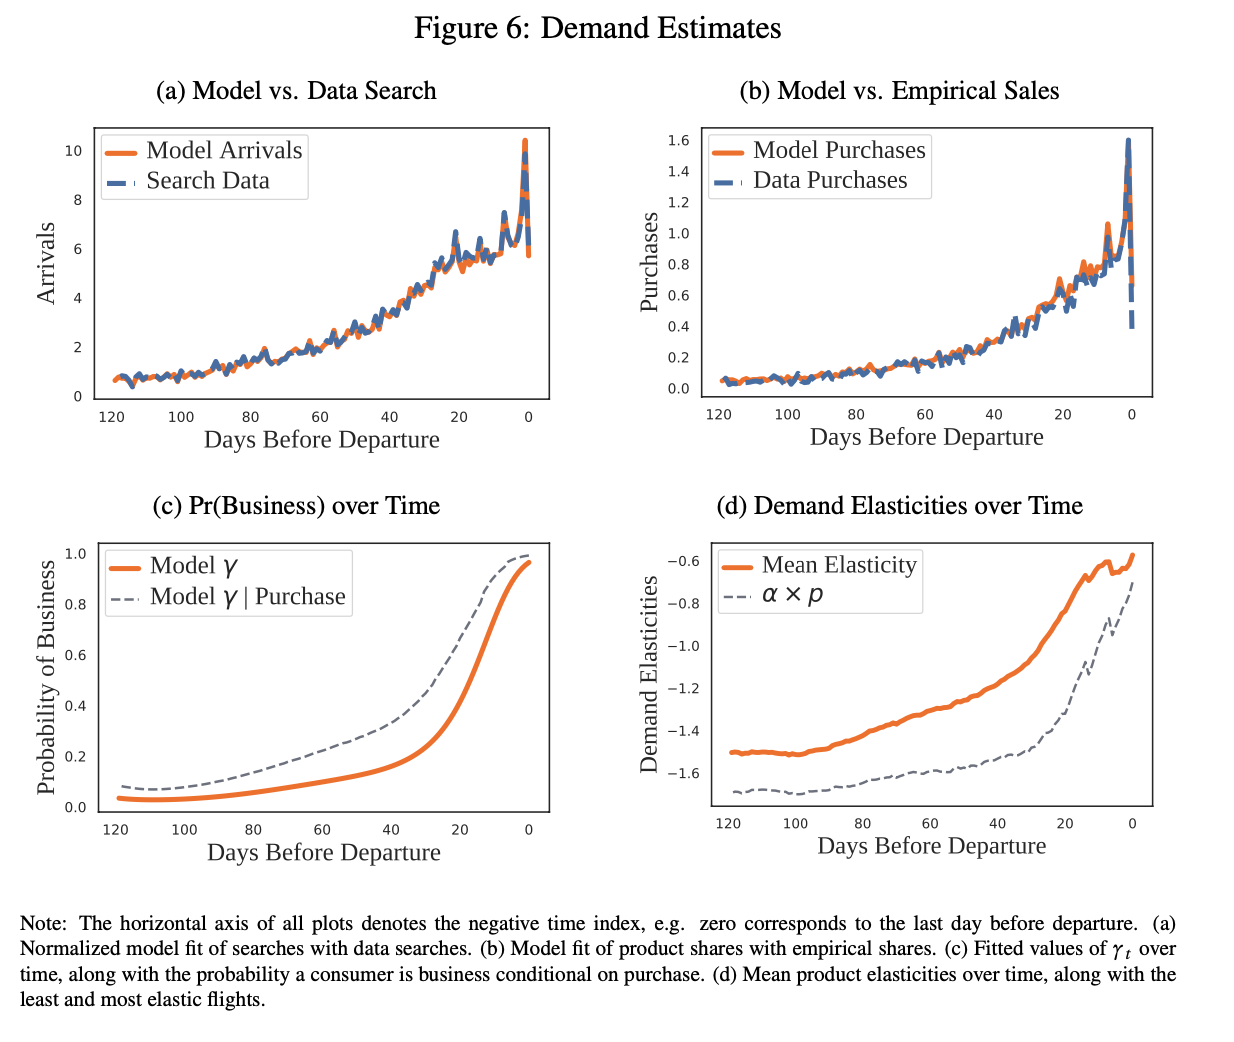
\includegraphics[width=\textwidth]{resources/williams_2023}      
\end{column}
\begin{column}{0.5\textwidth}
A nice extension/application of this approach
\begin{itemize}
    \item Consider high-frequency airline data where markets $M_t$ are \alert{small}
    \item Allow for poisson arrivals of consumers to the market who choose with mixed logit probabilities
    \item Not much individual data. Allow for business/leisure travelers (unobserved types)
    \item Mixture of Dirichlet Process for $(\xi, \omega)$
    \item One really good $z_{jt}$ (estimated shadow prices)
\end{itemize}
\end{column}
\end{columns}


\end{frame}

\section*{Combined Likelihood Approaches (GMPS 2023)}


\begin{frame}{Data}
    \begin{itemize}
        \item The researcher observes market-level data of purchases, and can construct market shares
    
            \begin{equation}
                s_{jm} = \frac{1}{N_m}\sum_{i=1}^{N_m}d_{ijm}
            \end{equation}
            
            where $N_m$ is the market size.
            
        \item For a subset of $S_m$ consumers (denoted by the dummy $D_{im}$) the researcher observes $\{(d_{i\cdot m},y_{im})\}$
    \end{itemize}
\end{frame}



\begin{frame}{Previous Approach: two-step estimator}

    \begin{itemize}
    
        \item Estimate $(\hat{\delta}, \hat{\theta})$ by maximizing the likelihood
        
        $$\mathcal{L}(\delta,\theta) =  \sum_i\sum_j\sum_m d_{ijm} \log \int \frac{\exp{(\delta_{jm} + \mu_{ijm}^{y} + \mu_{ijm}^{\nu})}}{\underbrace{\sum_{l=0}^{Jm}\exp{(\delta_{jm} + \mu_{ijm}^{y} + \mu_{ijm}^{\nu})}}_{s_{jm}(y_{im},\nu;\theta,\delta)}} dF(\nu)$$
        
        and recover $\hat{\beta}$ by running IV regression on $\hat{\delta}$.\\
        
        {\tiny Bayer, Ferreira, and McMillan (2007)\quad Bayer and Timmins (2007)}
        \item Uses only within-market variation to estimate $\theta$, which can break identification.
    
    \end{itemize}
\end{frame}


\begin{frame}{MDPLE estimator}

    \begin{itemize}
    
        \item GMPS 2023 propose the following estimator:
        
        \begin{equation}
            (\hat{\beta},\hat{\theta},\hat{\delta}) = \arg\min_{\beta,\theta,\delta} (\underbrace{-\log\hat{L}(\theta,\delta)+\hat{\Pi}(\beta,\delta)}_{\hat{\Omega}(\beta,\theta,\delta)})
        \end{equation}
        
        where
        
        \begin{enumerate}
            \item the \textbf{MDLE}
                \begin{align}
                    \log\hat{L}(\theta,\delta) =\sum_{m=1}^M\sum_{j=0}^{J_m}\sum_{i=1}^{N_m} d_{ijm}(D_{im}\log \pi_{jm}^{y_{im}}(\theta,\delta) + (1-D_{im})\log\pi_{jm}(\theta,\delta))\\
                     =\sum_{m=1}^M\sum_{j=0}^{J_m}\sum_{i=1}^{N_m} D_{im} d_{ijm} \log\frac{\pi_{jm}^{y_{im}}}{\pi_{jm}} + \sum_{m=1}^M N_m\sum_{j=0}^{J_m}s_{jm}\log\pi_{jm}
                \end{align}
                
                If $N_m = S_m$ this estimator $\leftrightarrow$ mixed-logit estimator in previous slides.\\
                If $S_m = 0$ maximizing the likelihood $\leftrightarrow$ imposing share constraints
        \end{enumerate}
    \end{itemize}

\end{frame}

\begin{frame}{MDPLE estimator (cont'd)}

    \begin{enumerate}
        \setcounter{enumi}{1}
        \item the \textbf{product level moments}
        \begin{equation}
            \hat{\Pi}(\beta,\delta) = \frac{1}{2}\hat{\mathcal{m}}^\intercal(\beta,\delta)\hat{\mathcal{W}}\hat{\mathcal{m}}^\intercal(\beta,\delta)
        \end{equation}
        where $\hat{\mathcal{m}}^\intercal(\beta,\delta) = \sum_{m=1}^M \sum_{j=1}^{J_m} b_{jm}(\delta_{jm}-\beta^\intercal x_{jm})$.\\
        
        If $d_b = d_\beta$ (exact identification) $\leftrightarrow$ two-step estimator\\
        If $d_b > d_\beta$ (overidentification): both terms contribute to the estimation of $\theta$, $\delta$
    \end{enumerate}
\end{frame}


\begin{frame}{Properties: efficiency}

\begin{itemize}
\item Show asymptotic equivalence of MDPLE with the GMM estimator

\begin{equation}
    (\hat{\beta},\hat{\theta},\hat{\delta}) = \arg\min_{\beta,\theta,\delta}\frac{1}{2}\begin{bmatrix}
\hat{\mathcal{m}}^\intercal & \partial_{\psi^\intercal}\log\hat{L}
\end{bmatrix}
\begin{bmatrix}
\hat{\mathcal{W}} & 0\\
0 & \hat{\mathcal{W}_L}
\end{bmatrix}
\begin{bmatrix}
\hat{\mathcal{m}} \\ \partial_{\psi}\log\hat{L}
\end{bmatrix}
\end{equation}

\item Show that the estimator above is efficient
\item  Trick: Also setup problem to be convex in $\delta$
\end{itemize}

\end{frame}

\begin{frame}{Properties: conformant convergence}
    
    \begin{itemize}
        \item Conformant: convergence rates adjust depending on alternative divergence rates of $\{N_m\}$, $S$, $J$ and variation in the data
        \item $\beta$ is identified only from $\hat{\Pi}$: convergence rate is always $\sqrt{J}$.
        \item Converge rates for $\theta$, $\delta$ depend on whether $\theta_z$ is fixed, and whether it is 0 or $\neq 0$.
        %\item If $\theta_z$ is fixed:
    \end{itemize}
    
    \begin{figure}[htbp]
    \begin{center}
    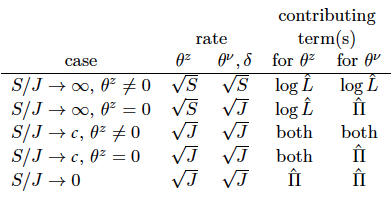
\includegraphics[width=.4\linewidth]{resources/conformant}
    \label{default}
    \end{center}
    \end{figure}

    \begin{itemize}
        \item Variation in the micro data alone is sufficient to identify $\theta_z$, $\theta^\nu$ and $\delta$ if the micro sample is large enough and demographic variation affects choice probabilities substantially.
    \end{itemize}
\end{frame}



% \begin{frame}{Comparisons}

% \begin{enumerate}

%     \item GMM version of the estimator (= MDLE replaced with score moments): asymptotically equivalent, but the GMM can suffer from the multiplicity of optima (while the MDLPE is convex in $\delta)$
%     \item imposing share constraints (BLP estimators): equivalent with MDLPE with infinite weights on some moments (loss of efficiency)
%     \item many micro moments in the literature (equivalent to approximated/linearized scores): slower convergence\\
%     \indent in the case of second choice data, expensive data is also a concern

% \end{enumerate}

% \end{frame}

\begin{frame}{Limitations of the MDPLE estimator}
    
    \begin{itemize}

        \item Incorporating supply-side moment conditions, or other moments that may make the MDPLE objective function non-convex.
        \item Limited gains compared to other approaches (in particular, the Optimal Micro BLP Estimator) when $\frac{S_m}{N_m}\to 0$ as $N\to\infty$.
        %\item Sometimes micro moments is all the researcher has access to!
        \item Assumes fully-compatible dataset (not true, e.g., if the researcher has censored data).
    \end{itemize}
\end{frame}



\section*{Micro BLP Approaches}

\begin{frame}{Micro BLP is used a lot}
    \vspace{0.5em}
    \scriptsize
    \begin{tabular}{rlrl}
        Paper & Industry & Paper & Industry \\
        \midrule
        \cite*{petrin2002quantifying} & Automobiles & \cite*{barwick2017local} & Automobiles \\
        \cite*{berry2004differentiated} & Automobiles & \cite*{murry2017advertising} & Automobiles \\
        \cite*{thomadsen2005effect} & Fast Food & \cite*{wollmann2018trucks} & Commercial Vehicles \\
        \cite*{goeree2008limited} & Personal Computers & \cite*{li2018better} & Automobiles \\
        \cite*{ciliberto2010public} & Cigarettes & \cite*{li2018empirical} & Digital Cameras \\
        \cite*{nakamura2010accounting} & Coffee & \cite*{backus2021common} & Cereal \\
        \cite*{beresteanu2011gasoline} & Automobiles & \cite*{grieco2021evolution} & Automobiles \\
        \cite*{li2012traffic} & Automobiles & \cite*{neilson2021targeted} & Primary Schools \\
        \cite*{copeland2014intertemporal} & Automobiles & \cite*{armitage2022regulatory} & Automobiles \\
        \cite*{starc2014insurer} & Health Insurance & \cite*{dopper2022rising} & Retail \\
        \cite*{ching2015quantifying} & Nursing Homes & \cite*{bodere2023dynamic} & Preschools \\
        \cite*{li2015price} & Automobiles & \cite*{montag2023mergers} & Laundry Machines \\
        \cite*{nurski2016exclusive} & Automobiles & \cite*{conlon2023market} & Distilled Spirits \\
        $\vdots$ & $\vdots$ & $\vdots$ & $\vdots$
    \end{tabular}
    \normalsize
    \vspace{0.5em}
    \begin{wideitemize}
        \item Many empirical IO papers use the ``micro BLP'' approach
        \begin{enumerate}
            \item Impose the \cite{berry1995automobile} share constraint (unlike {\color{lightgray}Grieco et al.\ 2023}) \nocite{grieco2023conformant}
            \item Stack product-level or ``\alert{aggregated}'' moments with ``\alert{micro}'' moments from consumer surveys
        \end{enumerate}
    \end{wideitemize}
\end{frame}

\begin{frame}{Towards a standardized framework}
    \begin{wideitemize}
        \item Despite the popularity of micro BLP, there's \alert{no standardized framework}
        \begin{itemize}
            \item Most papers use different notation to incorporate micro data in problem-specific ways
        \end{itemize}
                \item So econometric work is limited, with a few exceptions
        \begin{itemize}
            \item \cite{berry2014identification,berry2022nonparametric}: Nonparametric identification, including with micro data
            \item \cite{myojo2012asymptotic}: Extend \cite{berry2004limit} asymptotics to \cite{petrin2002quantifying}
        \end{itemize}
                \item We extend our BLP ``best practices'' \citep{conlon2020best} to the case with micro data
        \begin{enumerate}
            \item Provide a \alert{standardized framework} that covers most cases
            \item Derive \alert{practical advice} from econometrics, simulations, examples
            \item Make all this easy to do with \alert{PyBLP}
        \end{enumerate}
    \end{wideitemize}
\end{frame}

\begin{frame}[label=framework]{A standardized framework (Conlon Gortmaker 2023)}
    \begin{wideitemize}
        
        \item Aggregate data generated market-by-market $t$
        \begin{itemize}
            \item \alert{Products} $j \in \calJ_t$ have observed characteristics $x_{jt}$, unobserved quality $\xi_{jt}$
            \item \alert{Consumer types} $i \in \mathcal{I}_t$ have observed demographics $y_{it}$, unobserved preferences $\nu_{it}$
            \item \alert{Market shares} $s_{jt} = \sum_i w_{it} s_{ijt}$ integrate over consumer mass, each type has known weight $w_{it}$
        \end{itemize}
        
        \item Micro data generated dataset-by-dataset $d$, conditional on aggregate data
        \begin{itemize}
            \item Results $\{(t_n, j_n, y_{i_nt_n})\}_{n \in \mathcal{N}_d}$ from \alert{independent surveys} of \alert{selected consumers}
            \item Each consumer $n$ was surveyed with known probability $w_{di_nj_nt_n}$
        \end{itemize}
        
        \item Often only have or willing to use \alert{summary stats} (cost, compatibility, interpretability, etc.)
        \begin{itemize}
            \item Smooth functions $f(\overline{v}_d)$ of averages $\overline{v}_d = \frac{1}{N_d} \sum_n v_{di_nj_nt_n}$
        \end{itemize}
        
        \item \textit{``I want to match the mean demographic of consumers who purchased a product''}
        \begin{itemize}
            \item ``$\E[y_{it} \mid j \neq 0]$'' $\leftarrow$ Let $w_{dijt} = 1\{j \neq 0\}$ and $v_{dijt} = y_{it}$
        \end{itemize}
    \end{wideitemize}
\end{frame}



\begin{frame}[label=standard]{Standard micro moments}
    \begin{equation*}
        u_{ijt} = x_{jt}'(\beta_0 + \Pi_0 y_{it} + \Sigma_0 \nu_{it}) + \xi_{jt} + \varepsilon_{ijt}
    \end{equation*}
    
    \begin{wideitemize}
        \item With only product-level aggregate data, often difficult to accurately estimate $\Pi_0$ and $\Sigma_0$
        \begin{itemize}
            \item Often limited \alert{cross-market variation} in demographic distributions and choice sets
        \end{itemize}
        
        \item What \alert{within-market} micro variation is informative about $\Pi_0$?
        \begin{itemize}
            \item Literature tends to match stats that look like ``$\Cov(x_{jt}, y_{it} \mid j \neq 0)$''
        \end{itemize}
        
        \item What about $\Sigma_0$?
        \begin{itemize}
            \item Literature emphasizes \alert{second choices}, e.g.\ ``$\Cov(x_{jt}, x_{k(\text{-}j)t} \mid j, k \neq 0)$''
        \end{itemize}
        
        \item What about $\beta_0$?
        \begin{itemize}
            \item Only \alert{indirectly}: $\beta_0$ enters $s_{ijt}$ only through $\delta_{jt} = x_{jt}'\beta_0 + \xi_{jt}$, pinned down by share constraint
        \end{itemize}
    \end{wideitemize}
\end{frame}


\begin{frame}{Support for most cases}
    \vspace{0.5em}
    \scriptsize
    \begin{tabular}{@{\hspace{-1.2em}}r@{\hspace{0.6em}}l@{\hspace{-1.2em}}r@{\hspace{0.6em}}l@{\hspace{-1.2em}}}
        Paper & Micro moments shorthand & Paper & Micro moments shorthand \\
        \midrule
        \cite{petrin2002quantifying} & $\Pr(j \in \calJ \,|\, i \in \mathcal{I})$, $\E[y_i \,|\, j \in \calJ]$ & \cite{barwick2017local} & $\Pr(j \in \calJ \,|\, i \in \mathcal{I})$ \\
        {\color{lightgray}Berry et al.\ (2004)} & $\Cov(x_j, y_i \,|\, j \neq 0)$, $\Cov(x_j, x_{k(\text{-}j)} \,|\, j, k \neq 0)$ & \cite{murry2017advertising} & $\E[y_i \,|\, j \in \calJ]$ \\
        \cite{thomadsen2005effect} & $\Pr(j \in \calJ \,|\, i \in \mathcal{I})$ & \cite{wollmann2018trucks} & $\E[y_i \,|\, j \in \calJ]$ \\
        \cite{goeree2008limited} & $\Pr(j \in \calJ \,|\, i \in \mathcal{I})$ & \cite{li2018better} & $\Pr(j \in \calJ \,|\, i \in \mathcal{I})$ \\
        \cite{ciliberto2010public} & $\E[y_i \,|\, j \in \calJ]$ & \cite{li2018empirical} & $\Pr(j \in \calJ \,|\, i \in \mathcal{I})$ \\
        \cite{nakamura2010accounting} & $\Pr(j \in \calJ \,|\, i \in \mathcal{I})$ & \cite{backus2021common} & $\E[y_i \,|\, j \in \calJ]$, $\Cov(x_j, y_i \,|\, j \neq 0)$ \\
        \cite{beresteanu2011gasoline} & $\Pr(j \in \calJ \,|\, i \in \mathcal{I})$ & \cite{grieco2021evolution} & $\E[x_j \,|\, i \in \mathcal{I}, j \neq 0]$, $\Cov(x_j, x_{k(\text{-}j)} \,|\, j, k \neq 0)$ \\
        \cite{li2012traffic} & $\Pr(j \in \calJ \,|\, i \in \mathcal{I})$, $\E[y_i \,|\, j \in \calJ]$ & \cite{neilson2021targeted} & $\E[x_j \,|\, i \in \mathcal{I}, j \neq 0]$ \\
        \cite{copeland2014intertemporal} & $\E[y_i \,|\, j \in \calJ]$ & \cite{armitage2022regulatory} & $\E[y_i \,|\, j \in \calJ]$ \\
        \cite{starc2014insurer} & $\Pr(j \in \calJ \,|\, i \in \mathcal{I})$, $\E[x_j \,|\, i \in \mathcal{I}, j \neq 0]$ & \cite{dopper2022rising} & $\E[y_i \,|\, j \in \calJ]$ \\
        \cite{ching2015quantifying} & $\Pr(j \in \calJ \,|\, i \in \mathcal{I})$ & \cite{bodere2023dynamic} & $\Pr(j \in \calJ \,|\, i \in \mathcal{I})$, $\E[x_j \,|\, i \in \mathcal{I}, j \neq 0]$ \\
        \cite{li2015price} & $\Pr(j \in \calJ \,|\, i \in \mathcal{I})$ & \cite{montag2023mergers} & $\Cov(x_j, y_i \,|\, j \neq 0)$, $\Cov(x_j, x_{k(\text{-}j)} \,|\, j, k \neq 0)$ \\
        \cite{nurski2016exclusive} & $\E[y_i \,|\, j \in \calJ]$, $\Cov(x_j, y_i \,|\, j \neq 0)$ & \cite{conlon2023market} & $\E[y_i \,|\, j \in \calJ]$, $\E[x_j \,|\, i \in \mathcal{I}, j \neq 0]$ \\
        $\vdots$ & $\vdots$ & $\vdots$ & $\vdots$
    \end{tabular}
    \normalsize
    \vspace{0.5em}
    \begin{wideitemize}
        \item Framework supports most cases we've seen
        \begin{itemize}
            \item Demographic/choice-based sampling, conditioning, covariances, \alert{second choices} $k \neq j$ too!
        \end{itemize}
    \end{wideitemize}
\end{frame}


\begin{frame}[label=optimal]{Optimal micro moments}
    \begin{wideitemize}
        \item What in the full micro data $\{(t_n, j_n, y_{i_nt_n})\}_{n \in \mathcal{N}_d}$ is \alert{most informative} about $\theta_0$? The \alert{score}!
    \end{wideitemize}
    \begin{equation*}
        v_{ijt}(\theta_0) = \frac{\partial\log\Pr(t_n = t, j_n = j, y_{i_nt_n} = y_{it} \mid n \in \mathcal{N}_d)}{\partial\theta_0'}
    \end{equation*}
    
    \begin{wideitemize}
        \item Inspecting score expressions \alert{gives intuition} for which micro moments perform well
    \end{wideitemize}
    \begin{equation*}
        \hspace{2em}\underbrace{v_{ijt}(\Pi_0) \approx x_{jt} y_{it}}_{\mathclap{\textstyle\text{Similar to``$\Cov(x_{jt}, y_{it} \mid j \neq 0)$''}}} \hspace{6.5em} \underbrace{v_{ijkt}(\Sigma_0) \approx x_{jt} + x_{k(\text{-}j)t}}_{\mathclap{\textstyle\text{Similar to ``$\Cov(x_{jt}, x_{k(\text{-}j)t} \mid j, k \neq 0)$''}}} \hspace{4.5em} \underbrace{v_{ijt}(\beta_0) = 0}_{\mathclap{\textstyle\text{No direct info}}}
    \end{equation*}
    
    \begin{wideitemize}
        \item Feasible to match $v_{ijt}(\hat{\theta})$ at consistent $\hat{\theta}$ in second GMM step (with optimal weights/IVs)
        \begin{itemize}
            \item \alert{Asymptotically efficient} among all \alert{share-constrained} micro BLP estimators
            \item \alert{Computationally efficient} too, only need to compute scores once
            \item Must observe and be willing to use all info in the full micro data!
        \end{itemize}
    \end{wideitemize}
\end{frame}

\begin{frame}{Some words of caution}
    \begin{wideitemize}
        \item There are no efficiency guarantees for \alert{inconsistent} pilot estimates $\hat{\theta}$
        \begin{itemize}
            \item For first step, can use standard moments or score at informed guess of $\theta_0$
        \end{itemize}
        
        \item Most pairs of datasets have at least some  \alert{incompatibilities} in timing, variables, etc.
        \begin{itemize}
            \item Optimal micro moments will only work well if incompatibilities are small
            \item If large, match moments you expect to be compatible, e.g.\ correlations if scales are different
        \end{itemize}
    
        \item Quadrature behaves poorly with \alert{discontinuities} in moments like ``$\E[x_{jt} \mid y_{it} < \overline{y}, \, j \neq 0]$''
        \begin{itemize}
            \item Instead, use Monte Carlo methods or moments continuous in $y_{it}$ like ``$\Cov(x_{jt}, y_{it} \mid j \neq 0)$''
        \end{itemize}
    \end{wideitemize}
\end{frame}


\begin{frame}[label=estimator]{Micro BLP estimator}
    \vspace{-0.5em}
    \begin{equation*}
        \hat{\theta} = \argmin_\theta \hat{g}(\theta)'\hat{W}\hat{g}(\theta), \quad \hat{g}(\theta) =
        \begin{bmatrix}
            \hat{g}_\mathrm{A}(\theta) \\
            \hat{g}_\mathrm{M}(\theta)
        \end{bmatrix}
        =
        \begin{bmatrix}
            \frac{1}{N_\mathrm{A}} \sum_t \sum_j (\hat{\delta}_{jt}(\Pi, \Sigma) - x_{jt}'\beta) z_{jt} \\
            f_1(\overline{v}) - f_1(v(\Pi, \Sigma)) \\
            \vdots \\
            f_{M_\mathrm{M}}(\overline{v}) - f_{M_\mathrm{M}}(v(\Pi, \Sigma))
        \end{bmatrix}
    \end{equation*}
    \begin{wideitemize}
        \item \citepos*{berry1995automobile} share constraint gives mean utilities $\hat{\delta}_{jt}(\Pi, \Sigma)$
    \end{wideitemize}
    \begin{equation*}
        s_{jt} = \sum_i w_{it}  \frac{\exp[\hat{\delta}_{jt}(\Pi, \Sigma) + x_{jt}'(\Pi y_{it} + \Sigma \nu_{it})]}{1 + \sum_k \exp[\hat{\delta}_{kt}(\Pi, \Sigma) + x_{kt}'(\Pi y_{it} + \Sigma \nu_{it})]}
    \end{equation*}
    \begin{wideitemize}
        \item Micro moments $m$ match smooth functions $f_m(\cdot)$ of simple averages, called micro parts $p$
        \begin{equation*}
            \overline{v}_p = \frac{1}{N_{d_p}} \sum_n v_{pi_nj_nt_n} \xrightarrow{P_\mathrm{A}} v_p(\theta_0) = \E_\mathrm{A}[v_{pi_nj_nt_n}] = \frac{\sum_t \sum_i \sum_j w_{it} s_{ijt}(\theta_0) w_{d_pijt} v_{pijt}}{\sum_t \sum_i \sum_j w_{it} s_{ijt}(\theta_0) w_{d_pijt}}
        \end{equation*}
    \end{wideitemize}
\end{frame}



\begin{frame}{Simulations and asymptotics}
    \vspace{0.5em}
    \begin{wideitemize}
        \item Highlight this and other practical advice in Monte Carlo experiments
        \pause
        \item Study \alert{3 types of asymptotics}, punchline is that desirable properties translate to finite samples
    \end{wideitemize}
    \vspace{0.5em}
    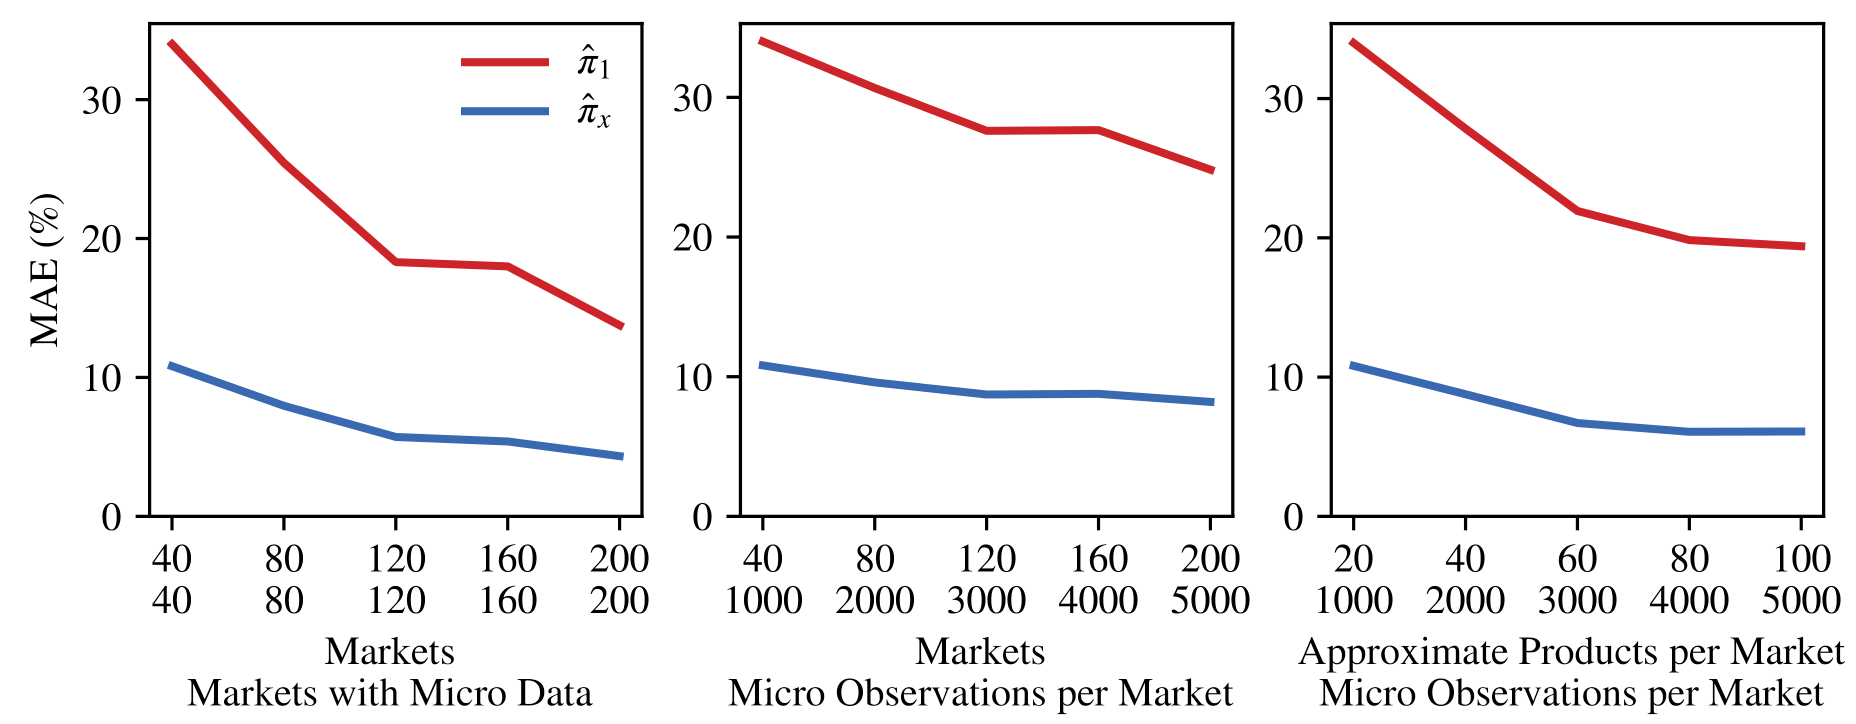
\includegraphics[width=0.95\textwidth]{simulations.png}
\end{frame}

\begin{frame}{Collecting second choices for an empirical example}
    \begin{columns}
        \begin{column}{0.75\textwidth}
            \vspace{0.5em}
            \begin{wideitemize}
                \item We demonstrate how all this works with \alert{Nielsen data}
                \begin{itemize}
                    \item Estimate pre-2017 demand for soft drinks in Seattle
                \end{itemize}
                \uncover<2->{
                    \item Counterfactual highlights \alert{diversion to the outside good}
                    \begin{itemize}
                        \item Predict effects of 2018 tax, compare with what happened ($-$22\%)
                    \end{itemize}
                }
                \uncover<3->{
                    \item So also show how to run cheap \alert{second choice survey}
                    \begin{itemize}
                        \item Diversion ratios discipline counterfactual in interpretable way
                    \end{itemize}
                }
            \end{wideitemize}
            \vspace{1em}
            \uncover<2->{
                \begin{tabular}{l@{\hspace{0.4em}}ccc}
                    \toprule
                    & Scanner Data & \& Household & \uncover<1,3->{\& Diversion} \\
                    \midrule
                    Taxed Volume Change (\%) & $-$30.1 & $-$30.0 & \uncover<1,3->{$-$16.5} \\
                    & \hspace{1em}(1.4) & \hspace{1em}(1.5) & \uncover<1,3->{\hspace{1em}(1.7)} \\
                    \addlinespace
                     High $-$ Low Income (pp) &  & \hspace{1em}2.0 & \uncover<1,3->{\hspace{1em}1.0} \\
                    & & \hspace{1em}(0.8) & \uncover<1,3->{\hspace{1em}(0.9)} \\
                    \bottomrule
                \end{tabular}
            }
        \end{column}%
        \begin{column}{0.25\textwidth}
            \vspace{1em}
            \uncover<3->{
                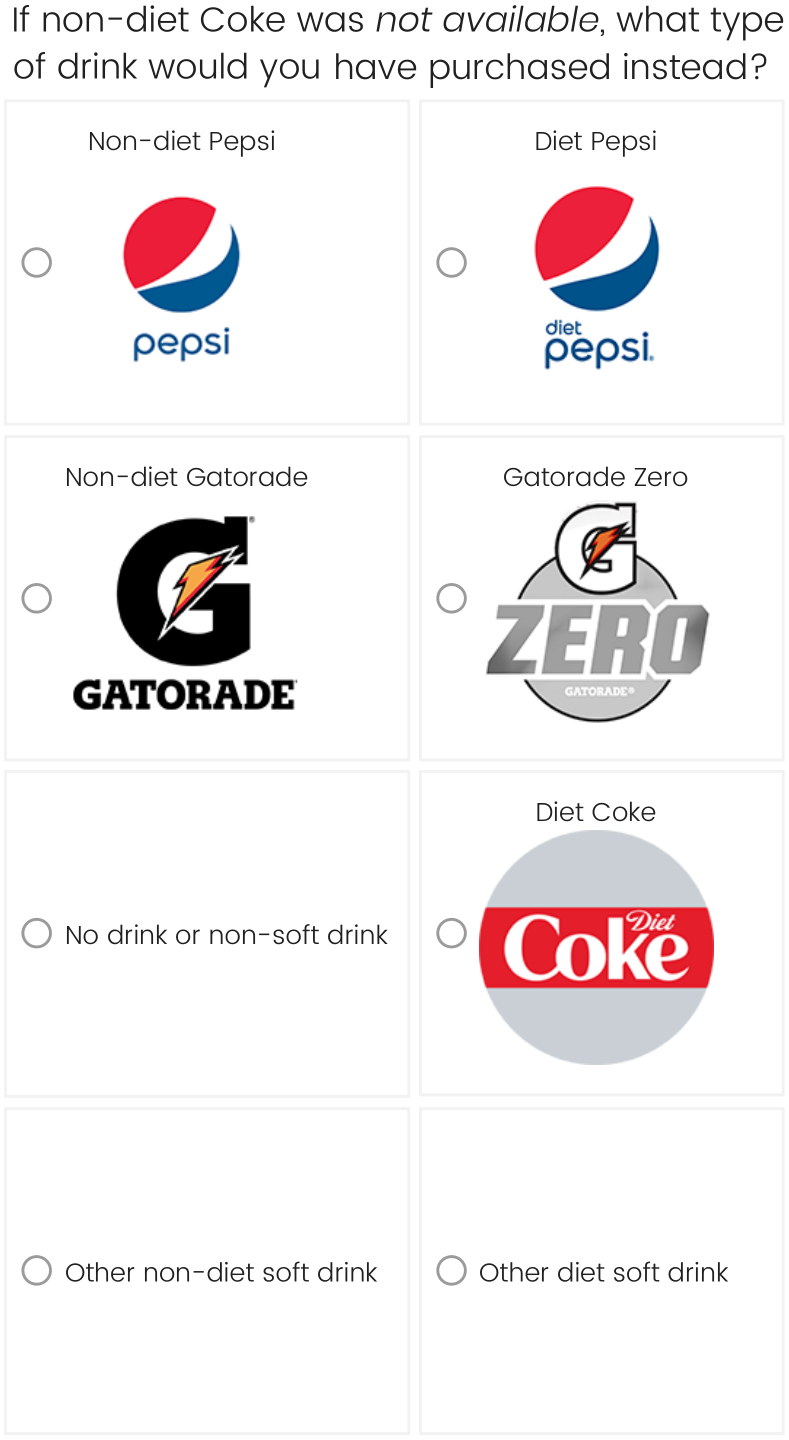
\includegraphics[width=\textwidth]{resources/survey.png}
            }
        \end{column}
    \end{columns}
\end{frame}

\begin{frame}{Replicating Petrin (2002) with PyBLP}
    \vspace{0.5em}
    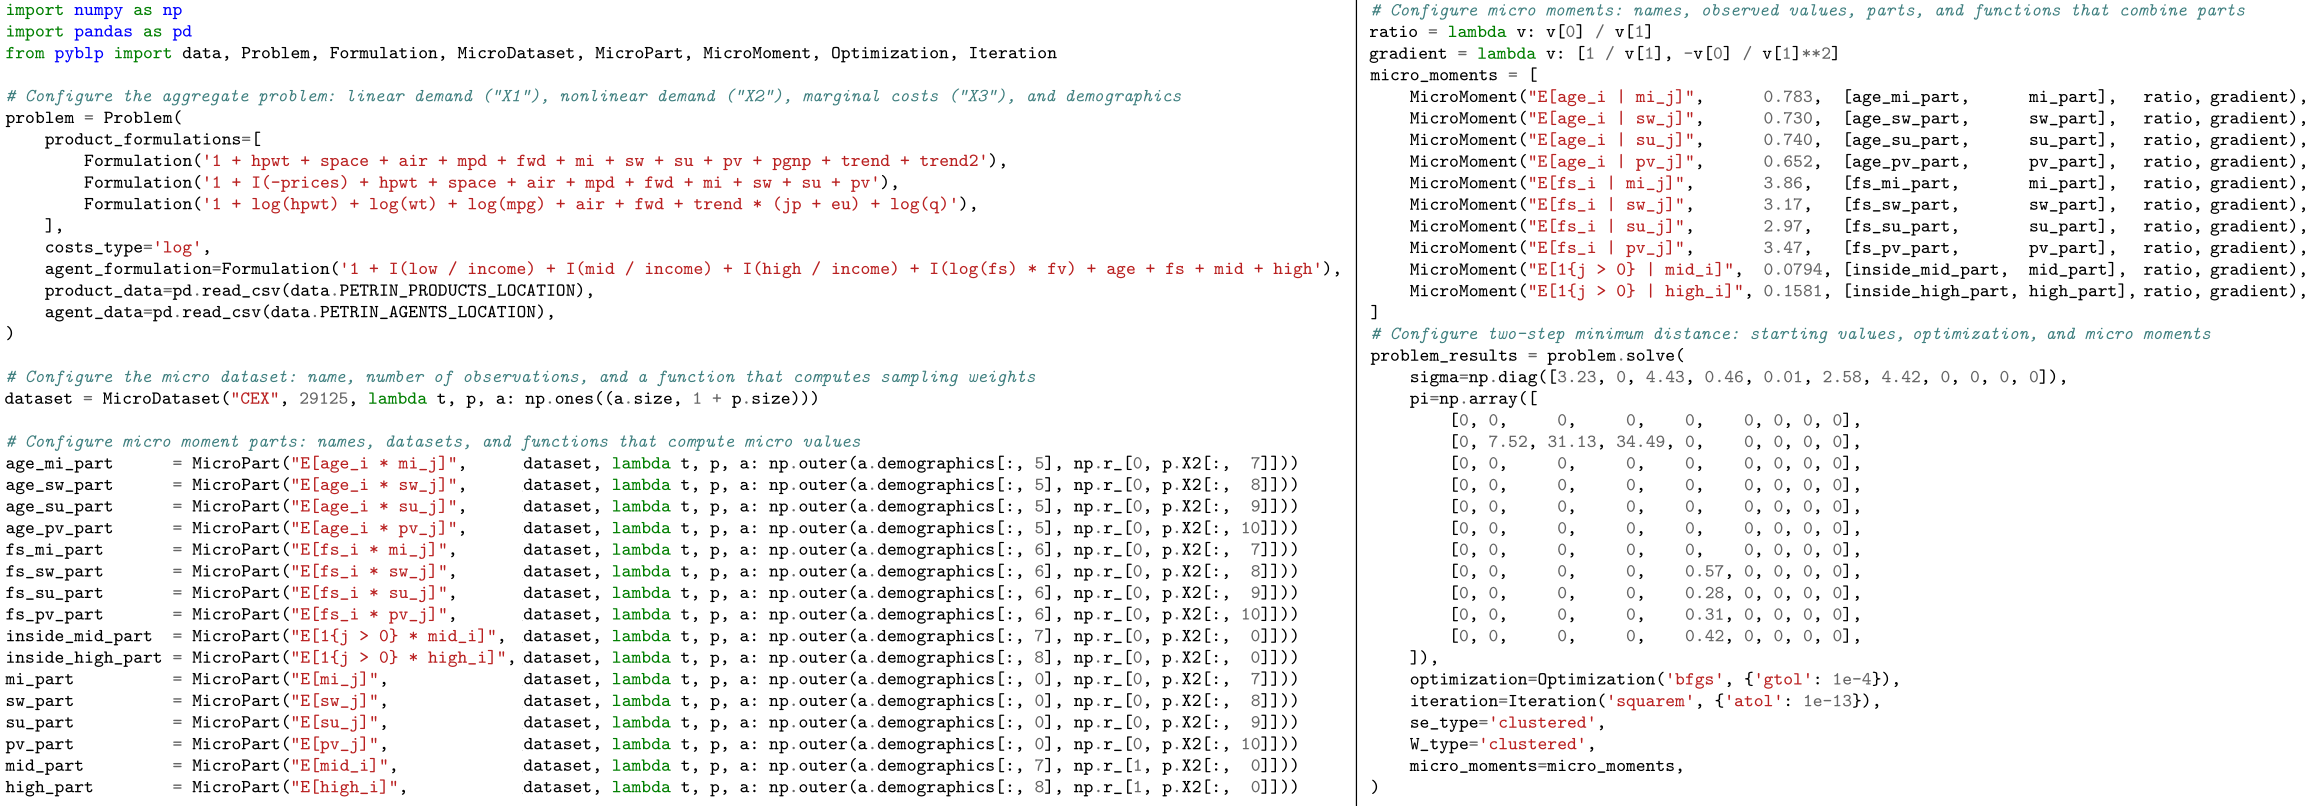
\includegraphics[width=\textwidth]{resources/petrin.png}
    \begin{wideitemize}
        \item We've tried our best to make all this easy to do with \alert{PyBLP}, including optimal micro moments
        \begin{itemize}
            \item E.g.\ can estimate \citepos{petrin2002quantifying} model with $<$ 100 lines of code
        \end{itemize}
    \end{wideitemize}
\end{frame}


\begin{frame}{Final Thoughts}
\begin{itemize}
    \item If you have relatively complete data on individual decisions, do MDLE
    \item If you have mostly aggregate data and some survey moments do microBLP.
    \item If you have very high-frequency data with lots of zeros, you are probably stuck doing some full likelihood Bayesian approach.
\end{itemize}
\end{frame}

\appendix

\begin{frame}[plain,allowframebreaks,noframenumbering]{References}
    \bibliography{references}
\end{frame}

\end{document}